\chapter[Capítulo 3. Background en algoritmos de árboles de decisión]{Background en algoritmos de árboles de decisión}

\section{Fundamentos de árboles de decisión}

 Los \textbf{árboles de decisión} \cite{ref3} son un tipo de algoritmos de aprendizaje supervisado (tanto para clasificación como para regresión) utilizado en diversos ámbitos como la inteligencia artificial, las finanzas, el marketing, etc. \\ Dado un conjunto de datos se fabrican diagramas de construcciones lógicas en forma de ramificaciones de árboles, muy similares a los sistemas de predicción basados en reglas, que sirven para representar y categorizar una serie de condiciones que ocurren de forma sucesiva, para la resolución de un problema.
 
 Adentrándonos en los aspectos más técnicos de este tipo de modelos de predicción, cabe destacar que las variables de entrada y de salida pueden ser tanto categóricas como continuas y que divide el espacio de los predictores (variables independientes) en regiones distintas y no superpuestas, tal como veremos en la siguiente figura.
 
 \begin{figure}[H]
 	\centering
 	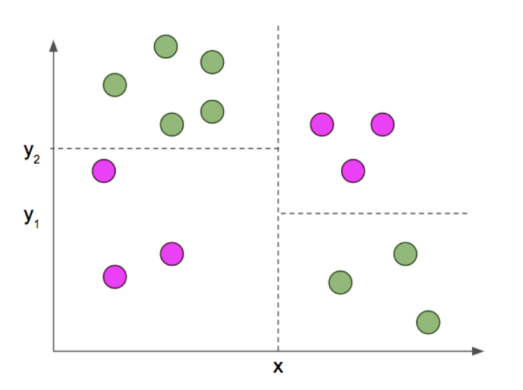
\includegraphics[width=0.7\textwidth]{imagenes/ejemploArboles} 
 	\caption{Ejemplo de árbol de decisión \cite{ref4}}
 \end{figure}
 
 Estas divisiones se realizan creando sobre la población (el conjunto de datos) subconjuntos lo más homogéneos posible entre las muestras que componen un grupo y lo más heterogéneo posible entre los distintos subconjuntos.\\
 Para la efectuación de esta separación, el algoritmo se basa en las variables de entrada más significativas, es decir, las que mejor separan las muestras.
 
 A continuación podemos observar las diferentes partes de un árbol de decisión.
 
  \begin{figure}[H]
 	\centering
 	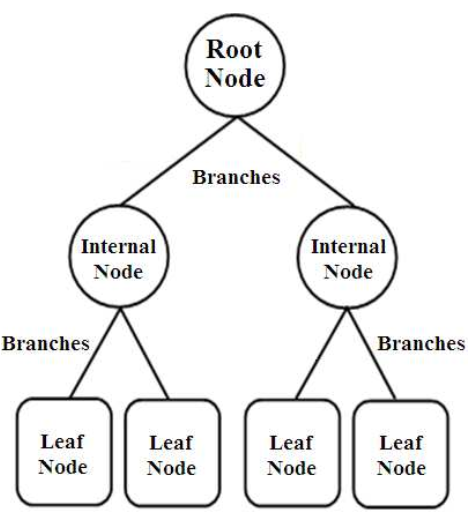
\includegraphics[width=0.5\textwidth]{imagenes/ejemploArbol} 
 	\caption{Partes de un árbol de decisión \cite{ref5}}
 \end{figure}

\textbf{Terminología:}
\begin{itemize}
	\item \textbf{Nodo raíz}: Es el primero de los nodos del árbol y forma la población completa.
	\item \textbf{Ramificación}: Son las ramas que conectan todos los nodos del árbol por donde pasan las muestras para ser clasificadas.
	\item \textbf{Nodo de decisión}: Son aquellos donde las muestras se evaluan para decidir por qué rama continuar el camino hacia la solución.
	\item \textbf{Nodo terminal/hoja}: Estos son los nodos solución, una vez la muestra llega a este tipo de nodo, el proceso de evaluación de esta ya ha finalizado, por lo que habrá sido clasificada en alguno de los grupos categóricos existentes.
	\item \textbf{Poda}: Consiste en cortar u obviar una rama del árbol en la evaluación de muestras, basándonos en cierta propiedad escogida, para evitar el recorrido del árbol completo y ahorrar de esta forma costos computacionales.
	\item \textbf{Rama/subárbol}: Es el conjunto de nodos y ramas completo que queda estrictamente por debajo de un nodo escogido del árbol total.
	\item \textbf{Nodos padre e hijo}: Dado un nodo del árbol, sus nodos hijo son todos aquellos que quedan conectados directamente a él únicamente en el nivel inferior siguiente. De esta forma, esos nodos hijo, comparten ese mismo padre.
\end{itemize}


\section{Hoeffding Trees y otros algoritmos de data streaming}

\section{Árboles de decisión monotónicos}


\newpage


